\subsection{Feature Extraction} \label{subsec:feature-extraction}

The feature extraction module receives a multi-channel audio signal of a fixed
length and outputs a \emph{feature frame}. Which is defined as the group of
vectors of features extracted from a finite number of samples. One vector per
\emph{extractor} used. \Cref{fig:datasets-frames} illustrates how an audio
signal is divided into frames.

\begin{figure}
    \centering
    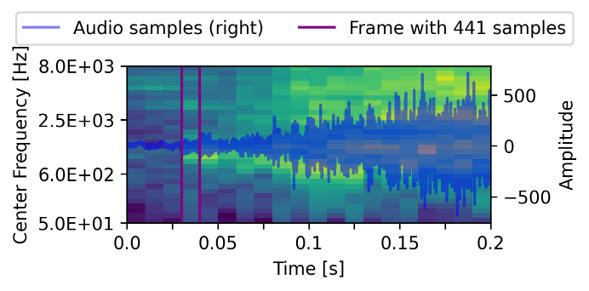
\includegraphics[width=\linewidth]{\subdir/frames.png}
    \caption[Audio frames]{Audio signal (in {\color{blue} blue}) over its
        features extracted from frames with a duration of 10ms with a single
        Gammatone filterbank extractor.}
    \label{fig:datasets-frames}
\end{figure}

The term \emph{extractor} will be used to abstract the system used to extract
features from audio data. This work opts to use a feature extractor based on
Gammatone filterbanks as \cite{marchegiani2018a} in since the performance of
classification systems relying on Mel Frequency Cepstrum Coefficients is
greatly reduced in the presence of noise. 

Gammatone filterbanks are an approximation to the human cochlear frequency
selectivity originally introduced in \cite{GTF1998}. Time-independent features
are obtained by filtering the audio waveform with a bank of gammatone band-pass
filters. 

This work implements a bank of fourth order gammatone filters with its
corresponding bandwidth of 1.019 ERB where ERB is the equivalent rectangular
bandwidth scale \cite{GLASBERG1990103}. The filters are linearly distributed
over a predefined frequency range on the ERB scale. The number of filters used
is equivalent to the number of features to be extracted. 